\subsection{Summary: Breaking the Three Walls}

This section addressed the three fundamental barriers to efficient MoE training, each a hard constraint that, unaddressed, prevents practical training at scale.

\begin{itemize}
    \item \textbf{Memory Wall}: Memory is the first constraint. If parameters, optimizer states, and activations exceed the GPU capacity, training cannot proceed. Memory-Efficient Permutation, FP8/FP4 activations, fine-grained recomputation, offloading, precision-aware optimizers, and FSDP together transform the 199.5 GB per-GPU requirement of DeepSeek-V3 into a feasible training configuration.

    \item \textbf{Communication Wall}: Communication overhead directly reduces GPU utilization. Optimized dispatchers (DeepEP, HybridEP) maximize bandwidth and FWD-BWD overlap hides latency behind computation. Together, these reduce all-to-all overhead from up to 60\% of the training time to less than 10\% in DeepSeek-V3 training.

    \item \textbf{Compute Efficiency Wall}: Compute inefficiency stems from two sources: small kernels that underutilize GPU resources, and host overhead that leaves GPUs idle. Grouped GEMM and kernel fusion improve kernel efficiency; CUDA Graphs and Sync-Free MoE eliminate host overhead. These transform computation inefficiency from the dominant bottleneck into a manageable constraint.
\end{itemize}

These optimizations are not independent. They form a coherent system where solutions to one wall enable or enhance solutions to others. Reduced-precision training shows this clearly: it reduces memory (activations) and improves compute efficiency (faster Tensor Core operations), while requiring careful integration to avoid introducing new bottlenecks (quantization kernel overhead).

The following sections address two cross-cutting concerns: Section~\ref{sec:reduced-precision-training} covers reduced-precision training in FP8/FP4, which simultaneously impacts all three walls, and Section~\ref{sec:long-context-training} addresses long-context MoE training, which changes the optimization balance when attention dominates computation.


%==============================================================================
% SECTION 5: Low PRECISION TRAINING - THE FP8 JOURNEY
%==============================================================================

\section{Reduced-Precision Training in FP8/FP4 for MoE}\label{sec:reduced-precision-training}

The preceding sections addressed each of the three walls with targeted optimizations. Reduced-precision training is unique: it simultaneously impacts memory, communication, and computation efficiency, making it a cross-cutting optimization that deserves dedicated treatment.

Mixed-precision training has been a cornerstone of efficient deep learning, with BF16 as standard practice \cite{micikevicius2018mixed,peng2023fp8lmtrainingfp8large,xi2024coat}. Reduced-precision training in FP8/FP4 represents a more aggressive step, reducing the precision from 16 bits to 8 or even 4, with correspondingly larger benefits and risks \cite{micikevicius2022fp8formatsdeeplearning,fishman2025scalingfp8trainingtrilliontoken}. For DeepSeek-V3, FP8 training reduces activation memory by approximately 16 GB per GPU, improves expert GEMMs through faster Tensor Core operations, and accelerates the parameter AllGather communication. These gains compound across the three walls, making FP8 essential for efficient large-scale MoE training.

However, low-precision training introduces convergence risks that must be systematically addressed. This section presents Megatron-Core's approach to reduced-precision training: understanding where precision matters, selecting appropriate quantization recipes, and implementing MoE-specific optimizations that capture benefits of reduced-precision training while maintaining training stability.

\subsection{Why Reduced-Precision Training Matters for MoE}\label{sec:precision-anatomy}

MoE architectures amplify both the benefits and risks of low-precision training compared to dense models:

\textbf{Amplified Benefits.} With hundreds of experts, activation memory scales proportionally. FP8/FP4 activations provide larger absolute memory savings than in dense models. The communication volume for parameter AllGather is halved\footnote{For the NVFP4 recipe on Blackwell, since we need to gather both the row-wise and column-wise weight tensors, the saved communication volume is also 50\%.}, and expert GEMMs (which dominate MoE computation) benefit from faster Tensor Core throughput.

\textbf{Amplified Risks.} Router decisions depend on precise scores to assign tokens to experts. Quantization noise could destabilize expert selection, leading to training instability, degraded model quality, or expert collapse \cite{nagel2021whitepaper}. The numerically sensitive components must be protected from aggressive quantization.

\textbf{The Strategy: Selective Precision.} The solution is precision where it matters, efficiency everywhere else. Three principles guide the deployment of reduced-precision training in MoE:
\begin{enumerate}
    \item \textbf{Protect routing decisions.} The router remains in FP32 to ensure stable expert selection.
    \item \textbf{Preserve precision for key components.} Embeddings, output layers, main gradients, master weights, and optimizer states remain in their original precision to maintain model quality.
    \item \textbf{Quantize bulk computation.} Expert GEMMs, which constitute the majority of computation, use reduced-precision training with carefully designed quantization schemes (called \textit{recipe}).
\end{enumerate}

\begin{notebox}
The key to successful reduced-precision MoE training is selective precision: keep numerically sensitive components (router, embeddings, output layers, gradients, and optimizer states) in higher precision while aggressively quantizing the bulk of computation (expert GEMMs). This strategy captures most benefits of the reduced-precision training while avoiding convergence issues.
\end{notebox}

\subsection{The Impact from Reduced-Precision Training on All Three Walls}

Reduced-precision training provides benefits across all three performance walls, making it a unifying optimization. Table~\ref{tab:fp8-impact-summary} summarizes these impacts.

\begin{table}[ht]
\centering
\begin{threeparttable}
\caption{Summary of the impact from reduced-precision training on the Three Walls.}
\label{tab:fp8-impact-summary}
\begin{tabular}{lll}
\toprule
\textbf{Wall} & \textbf{Reduced-Precision Training Benefit} & \textbf{Details} \\
\midrule
Memory & 50\% (FP8)/75\% (FP4) activation reduction & Section~\ref{sec:fp8-activation} \\
        & Eliminate BF16 weight copies & Section~\ref{subsec:fp8-primary-weights} \\
        & BF16 optimizer states & Section~\ref{sec:precision-opt} \\
\midrule
Communication & 50\% parameter AllGather \tnote{1} & Section~\ref{subsec:fp8-primary-weights} \\
\midrule
Compute & Faster Tensor Core GEMMs & Section~\ref{sec:fp8-training} \\
        & Quantization kernel overhead & Section~\ref{sec:kernel-fusion} \\
\bottomrule
\end{tabular}
\begin{tablenotes}
    \footnotesize
    \item[1] For NVFP4, we need to gather both row-wise and column-wise FP4 weights, so the reduced traffic of parameter AllGather is also 50\%.
\end{tablenotes}
\end{threeparttable}
\end{table}

\subsubsection{Breaking the Memory Wall with Reduced-Precision Training}

Reduced-precision training reduces memory consumption in three ways:

\textbf{Activation Memory (detailed in Section~\ref{sec:fp8-activation}).} The primary source of activation memory savings comes from input tensors of linear layers saved for backward computation. By storing these tensors in FP8/FP4 instead of BF16, the memory footprint is reduced by 50\%/75\%. For example, FP8 saves approximately 16 GB of activation memory per GPU for DeepSeek-V3.

\textbf{Parameter Memory.} Conventional reduced-precision training maintains three parameter copies: FP32 master weights, BF16 model weights, and FP8/FP4 computation weights. Our \emph{native FP8/FP4} approach (detailed in Section~\ref{subsec:fp8-primary-weights} below) eliminates the BF16 copy by casting weights directly from FP32 to FP8/FP4 and doing parameter AllGather in reduced precisions.

\textbf{Optimizer State Memory (detailed in Section~\ref{sec:precision-opt}).} Adam optimizer states (first and second moments) can be stored in BF16 instead of FP32, reducing optimizer memory by 50\%. This is orthogonal to reduced-precision training and is also applicable to BF16.

\subsubsection{Breaking the Communication Wall with Reduced-Precision Training}
\label{sec:comm_wall_quantized_training}

% \textbf{FP8 EP Dispatch (detailed in Section~\ref{sec:fp8-dispatch-comm}).} For fine-grained MoE models with large EP sizes, all-to-all communication becomes a primary bottleneck. By dispatching tokens in FP8 instead of BF16, the communication volume is halved. The key challenge is managing the dequantization-quantization cycle required because forward and backward passes use different quantization dimensions.

\textbf{Parameter AllGather in FP8/FP4.} When using FP8/FP4 primary weights with distributed optimizer, parameter AllGather communication is reduced by 50\% (1 byte vs 2 bytes per parameter). Note that
\begin{itemize}
    \item For NVFP4, we need to gather both row-wise and column-wise FP4 weights, so the reduced traffic of parameter AllGather is also 50\%.
    \item For MXFP8, even with FP8 primary weights, we first copy the FP32 master weights into a temporary BF16 buffer and communicate in BF16 precision. This is because MXFP8 requires different quantization directions for forward and backward passes. Communicating MXFP8 weights would require both row-wise and column-wise quantized versions, effectively communicating two bytes per parameter and eliminating any advantage over communicating BF16. Hence, for MXFP8, we communicate parameters in BF16 precision. 
\end{itemize}

\subsubsection{Breaking the Compute Efficiency Wall with Reduced-Precision Training}

\textbf{Faster GEMMs.} FP8 (Ada/Hopper and later) and FP4 (Blackwell and later) Tensor Cores provide higher throughput than BF16, accelerating both forward and backward passes.

\textbf{The Trade-off: Quantization Overhead.} Reduced-precision training introduces additional quantization kernels that increase CPU overhead, which is particularly problematic for fine-grained MoE where many small operations already stress the CPU. This overhead is managed through:
\begin{itemize}
    \item \textbf{Kernel fusion} that fuses quantization with other operations, such as normalization and activation functions.
    \item \textbf{Fuse padding/unpadding} with the permutation kernel or routing map to avoid explicit padding/unpadding.
    \item \textbf{Grouped quantization} that fuses the quantization of multiple input tensors into one single kernel.
    \item \textbf{CUDA Graphs} that captures quantization kernels to eliminate launch overhead. See Section~\ref{sec:cuda-graphs} for more details.
\end{itemize}

\subsection{Reduced-Precision Training Recipes: Per-Tensor FP8, Blockwise FP8, MXFP8, and NVFP4}

Having established the impact of reduced-precision training on all three walls, we now examine the technical components that define a reduced-precision training configuration.

\begin{figure}[ht]
    \centering
    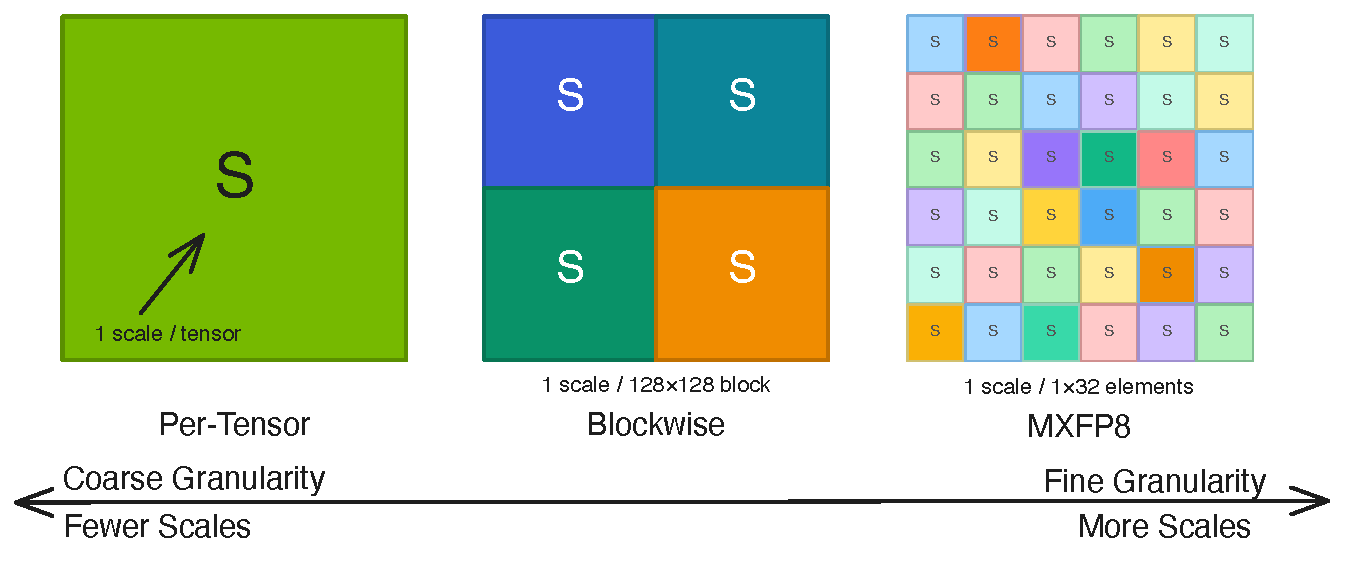
\includegraphics[width=0.9\textwidth]{figures/plots/fp8_recipes_comparison_draft.pdf}
    \caption{FP8 training recipes: Per-Tensor Scaling, Blockwise FP8, and MXFP8.}
    \label{fig:fp8-recipes-overview}
\end{figure}

A reduced-precision training recipe consists of:
\begin{itemize}
    \item \textbf{Data format.} There are two types of FP8 format: E4M3 and E5M2 \cite{micikevicius2022fp8formatsdeeplearning,kuzmin2022fp8quantization}. Usually there are two combinations used in training:
    \begin{itemize}
        \item \textbf{E4M3}: Inputs, weights, and gradients are all quantized in the E4M3 format.
        \item \textbf{Hybrid}: Inputs and weights are quantized in E4M3, while gradients are quantized in E5M2.
    \end{itemize}
    While for FP4, E2M1 is the only supported format.
    \item \textbf{Scaling granularity.} Choices include per-tensor and per-block (also called group or tile). For per-block scaling, the block size also varies between recipes.
    \item \textbf{Which parts are quantized.} Usually all linear layers are quantized, while keeping embedding, output layer (LM head), and optimizers in their original high precision. Part of the communication can be in FP8/FP4 (e.g., TP AllGather, DP AllGather, EP all-to-all). Current reduced-precision training recipes usually keep SDPA in BF16.
    \item \textbf{Additional mechanisms}, such as stochastic rounding, Random Hadamard Transforms (RHT), etc. These mechanisms are recipe-specific and require careful verification. 
\end{itemize}

Megatron-Core provides three FP8 recipes, each validated at scale (\figref{fig:fp8-recipes-overview}). The evolution from per-tensor to blockwise to MXFP8 reflects both hardware advances and lessons learned from large-scale deployments. \textbf{Per-Tensor Scaling} uses a single scale factor per tensor, simple but limited precision, suitable for experimentation. \textbf{Blockwise FP8} (128$\times$128 blocks) provides finer granularity with proven stability at scale, recommended for Hopper. \textbf{MXFP8} (1$\times$32 granularity) offers native Blackwell Tensor Core support with hardware-accelerated scaling, recommended for Blackwell. Besides, Megatron-Core also provides an NVFP4 recipe \cite{nvidia2025pretraininglargelanguagemodels} on Blackwell.

\subsubsection{Per-Tensor FP8 Recipe}
The per-tensor FP8 recipe, supported on Hopper and Blackwell, usually adopts the hybrid format (E4M3 for inputs/weights, E5M2 for gradients). It calculates the absolute max value (amax) of all values in the input tensor and uses that to quantize the tensor into FP8.

There are two variants of per-tensor scaling:
\begin{itemize}
    \item \textbf{Delayed scaling}: Use the amax from a history window. This breaks the data dependency between the calculation of amax and scaling, offering the best performance at the risk of losing precision due to the estimated amax.
    \item \textbf{Current (live) scaling}: Calculate the amax in a just-in-time manner, providing better precision.
\end{itemize}

We do not recommend delayed scaling due to precision issues; current scaling provides better precision and model convergence.
Figures~\ref{fig:fp8-cs-hopper} and~\ref{fig:fp8-cs-blackwell} illustrate the computation of a linear layer with per-tensor current scaling on the Hopper and Blackwell platforms, respectively. Since only TN layout FP8 GEMM is supported on Hopper, we must store the transposed FP8 activations for backward calculation. In Transformer Engine, the quantization kernels fuse the cast and transpose into a single kernel to reduce global memory access. On the Blackwell platform, FP8 GEMMs in all layouts are supported, so we do not need the transposed version, further reducing the memory footprint.

Per-tensor scaling is a good starting point for migrating to FP8 training due to its simplicity and relatively good precision and performance.


\begin{figure*}[t!]
    \centering
    \begin{subfigure}[t]{0.45\textwidth}
        \centering
        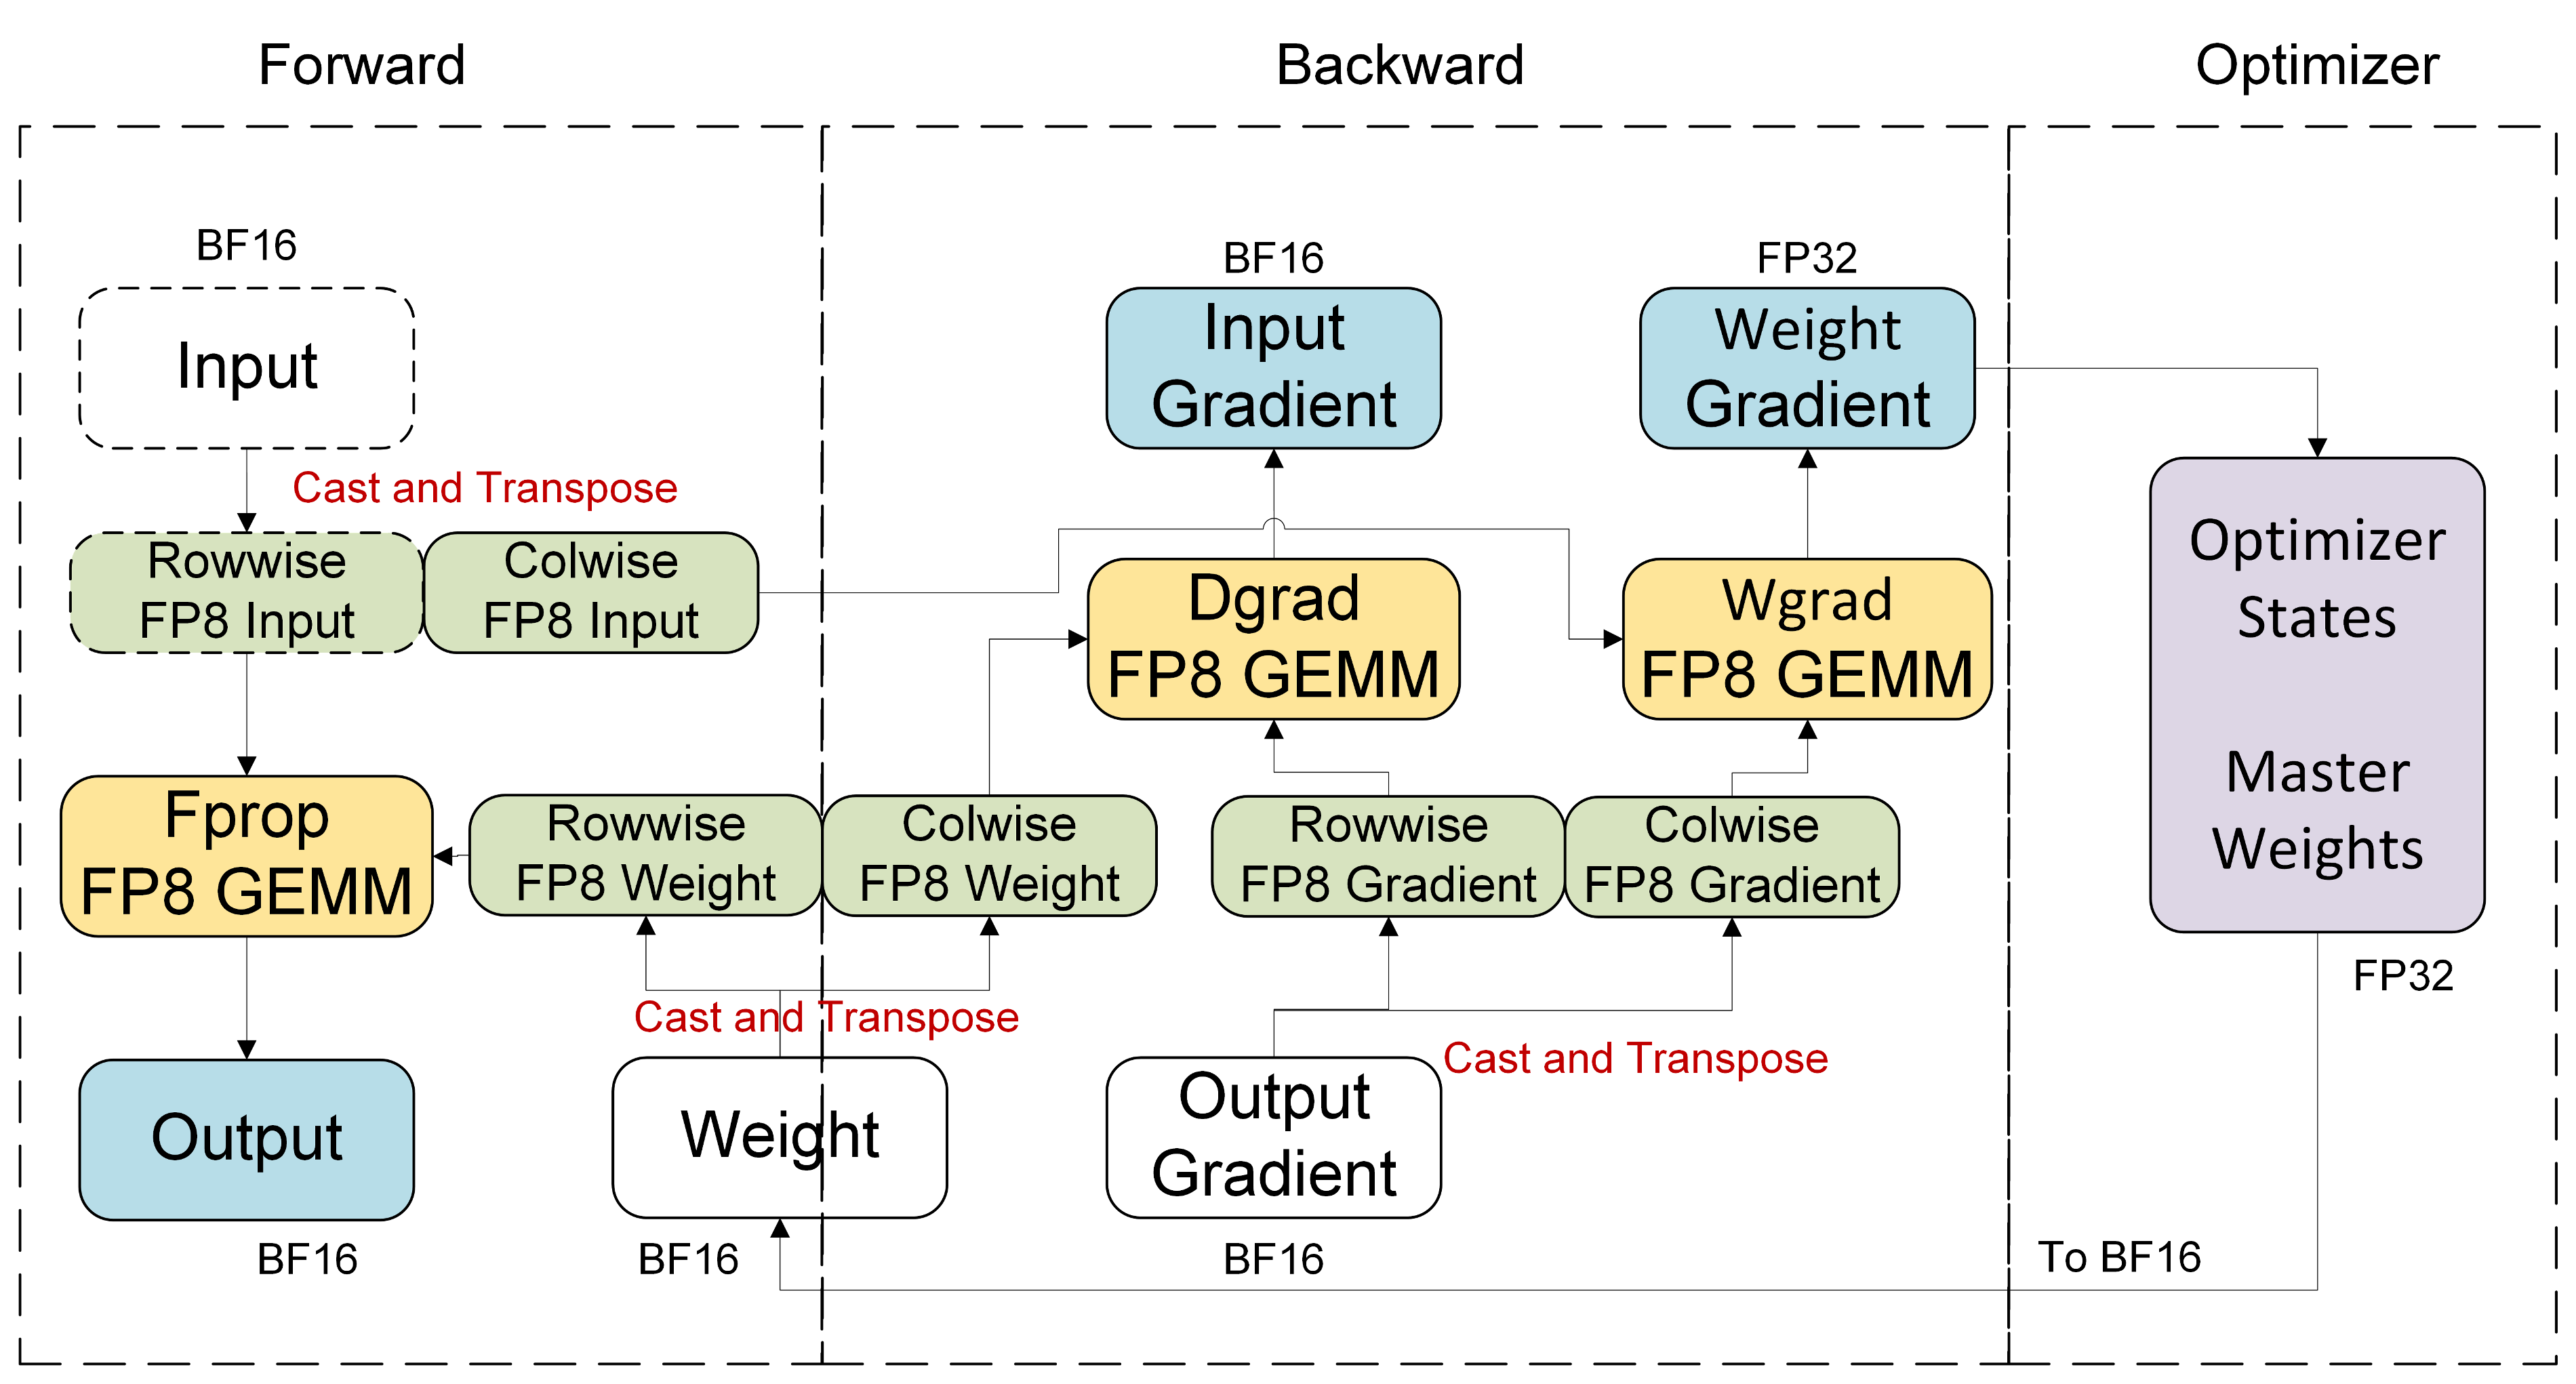
\includegraphics[width=1.0\linewidth]{figures/fp8-cs-hopper.png}
        \caption{Per-tensor Current scaling on the Hopper platform.}
        \label{fig:fp8-cs-hopper}
    \end{subfigure}
    \begin{subfigure}[t]{0.45\textwidth}
        \centering
        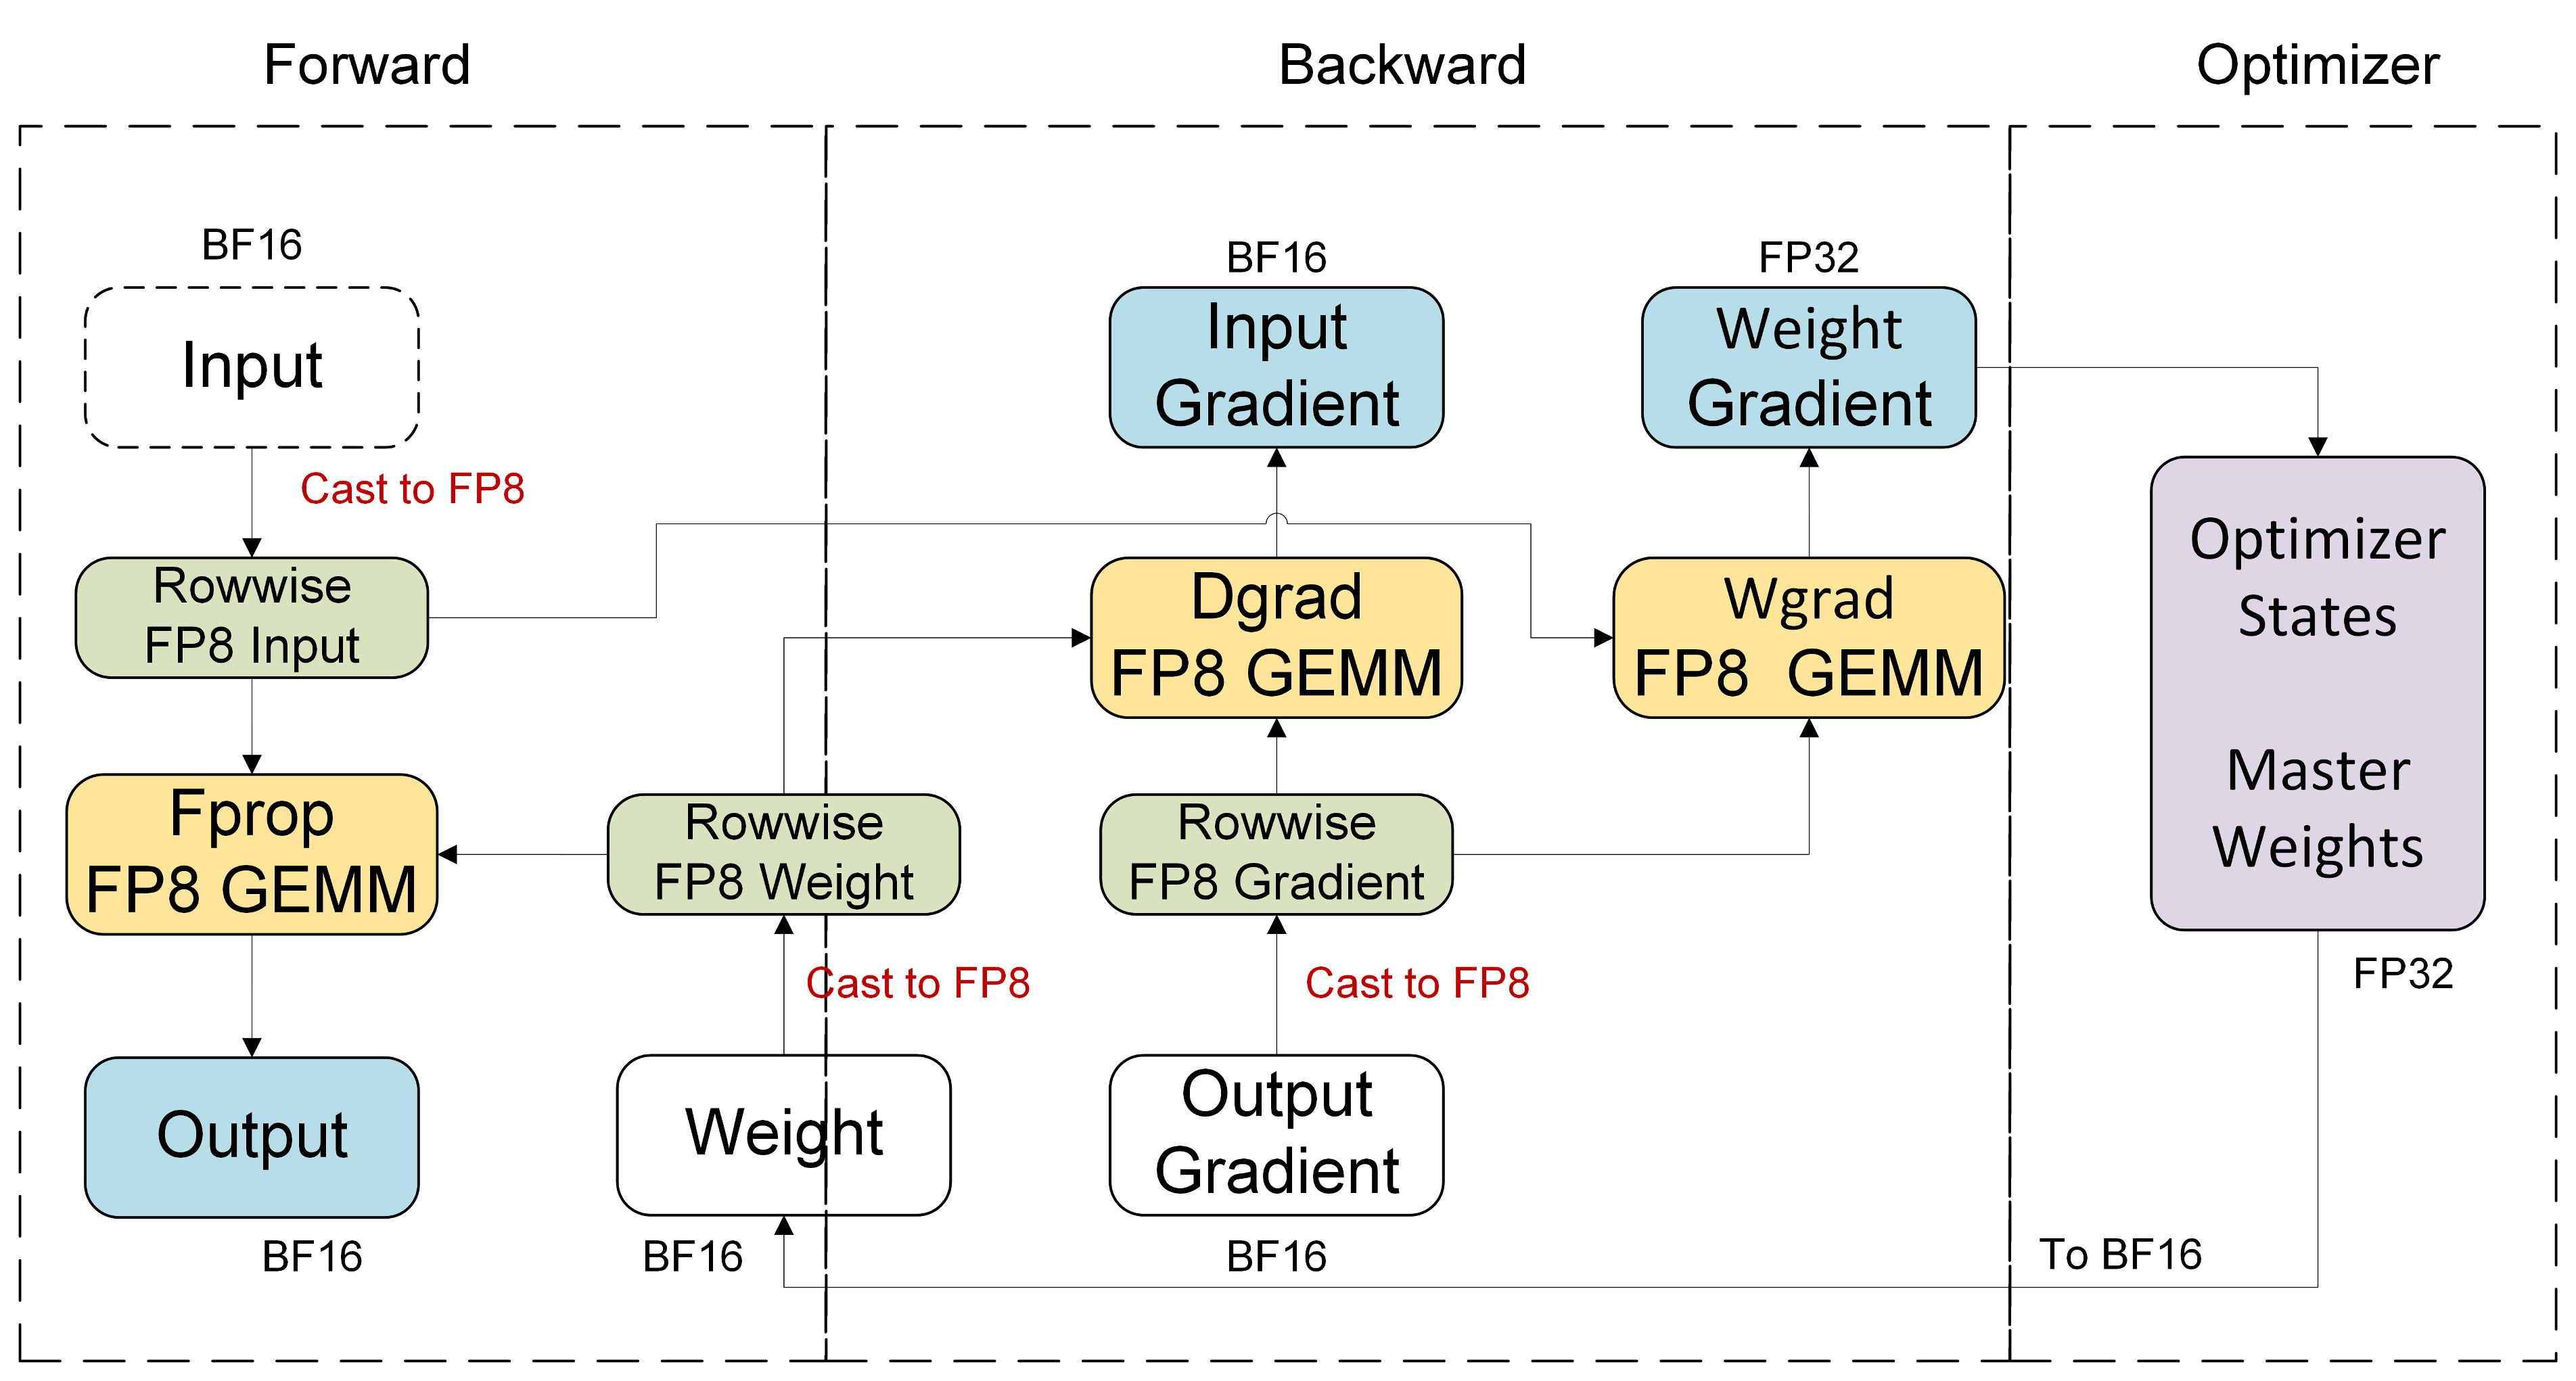
\includegraphics[width=1.0\linewidth]{figures/fp8-cs-blackwell.png}
        \caption{Per-tensor Current scaling on the Blackwell platform.}
        \label{fig:fp8-cs-blackwell}
    \end{subfigure}
    \begin{subfigure}[t]{0.45\textwidth}
        \centering
        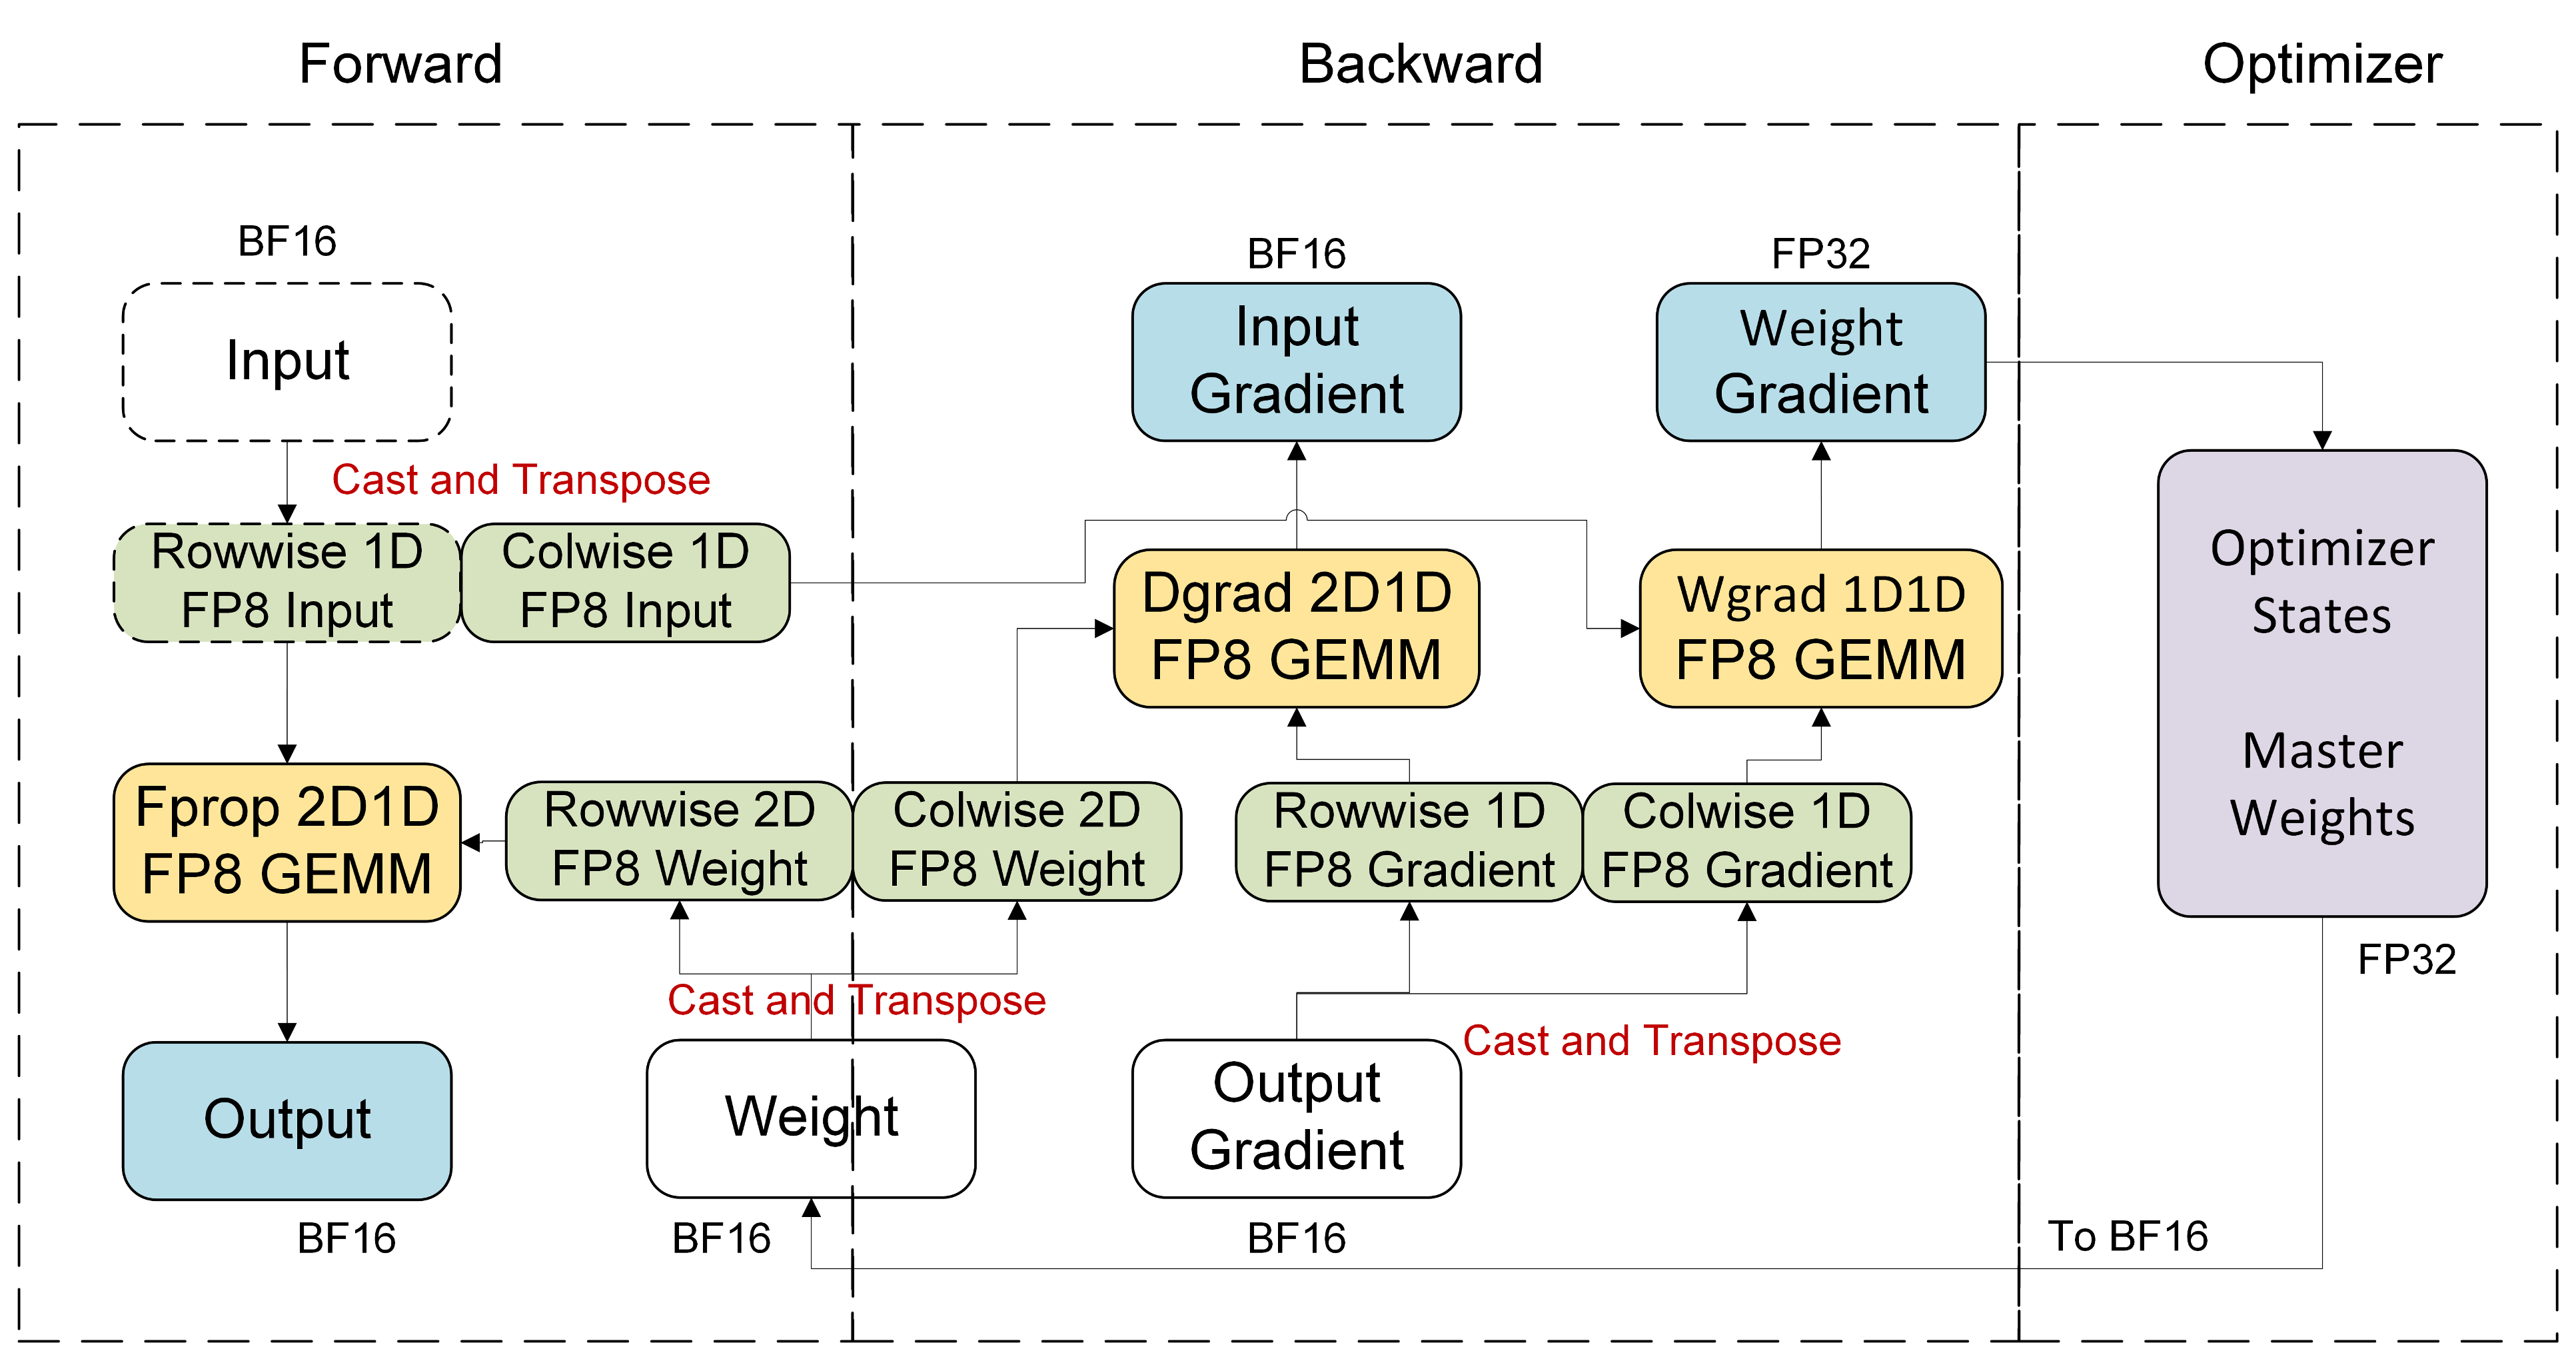
\includegraphics[width=1.0\linewidth]{figures/fp8-blockwise-hopper.png}
        \caption{Blockwise FP8 recipe on Hopper.}
        \label{fig:fp8-blockwise-hopper}
    \end{subfigure}
    \begin{subfigure}[t]{0.45\textwidth}
        \centering
        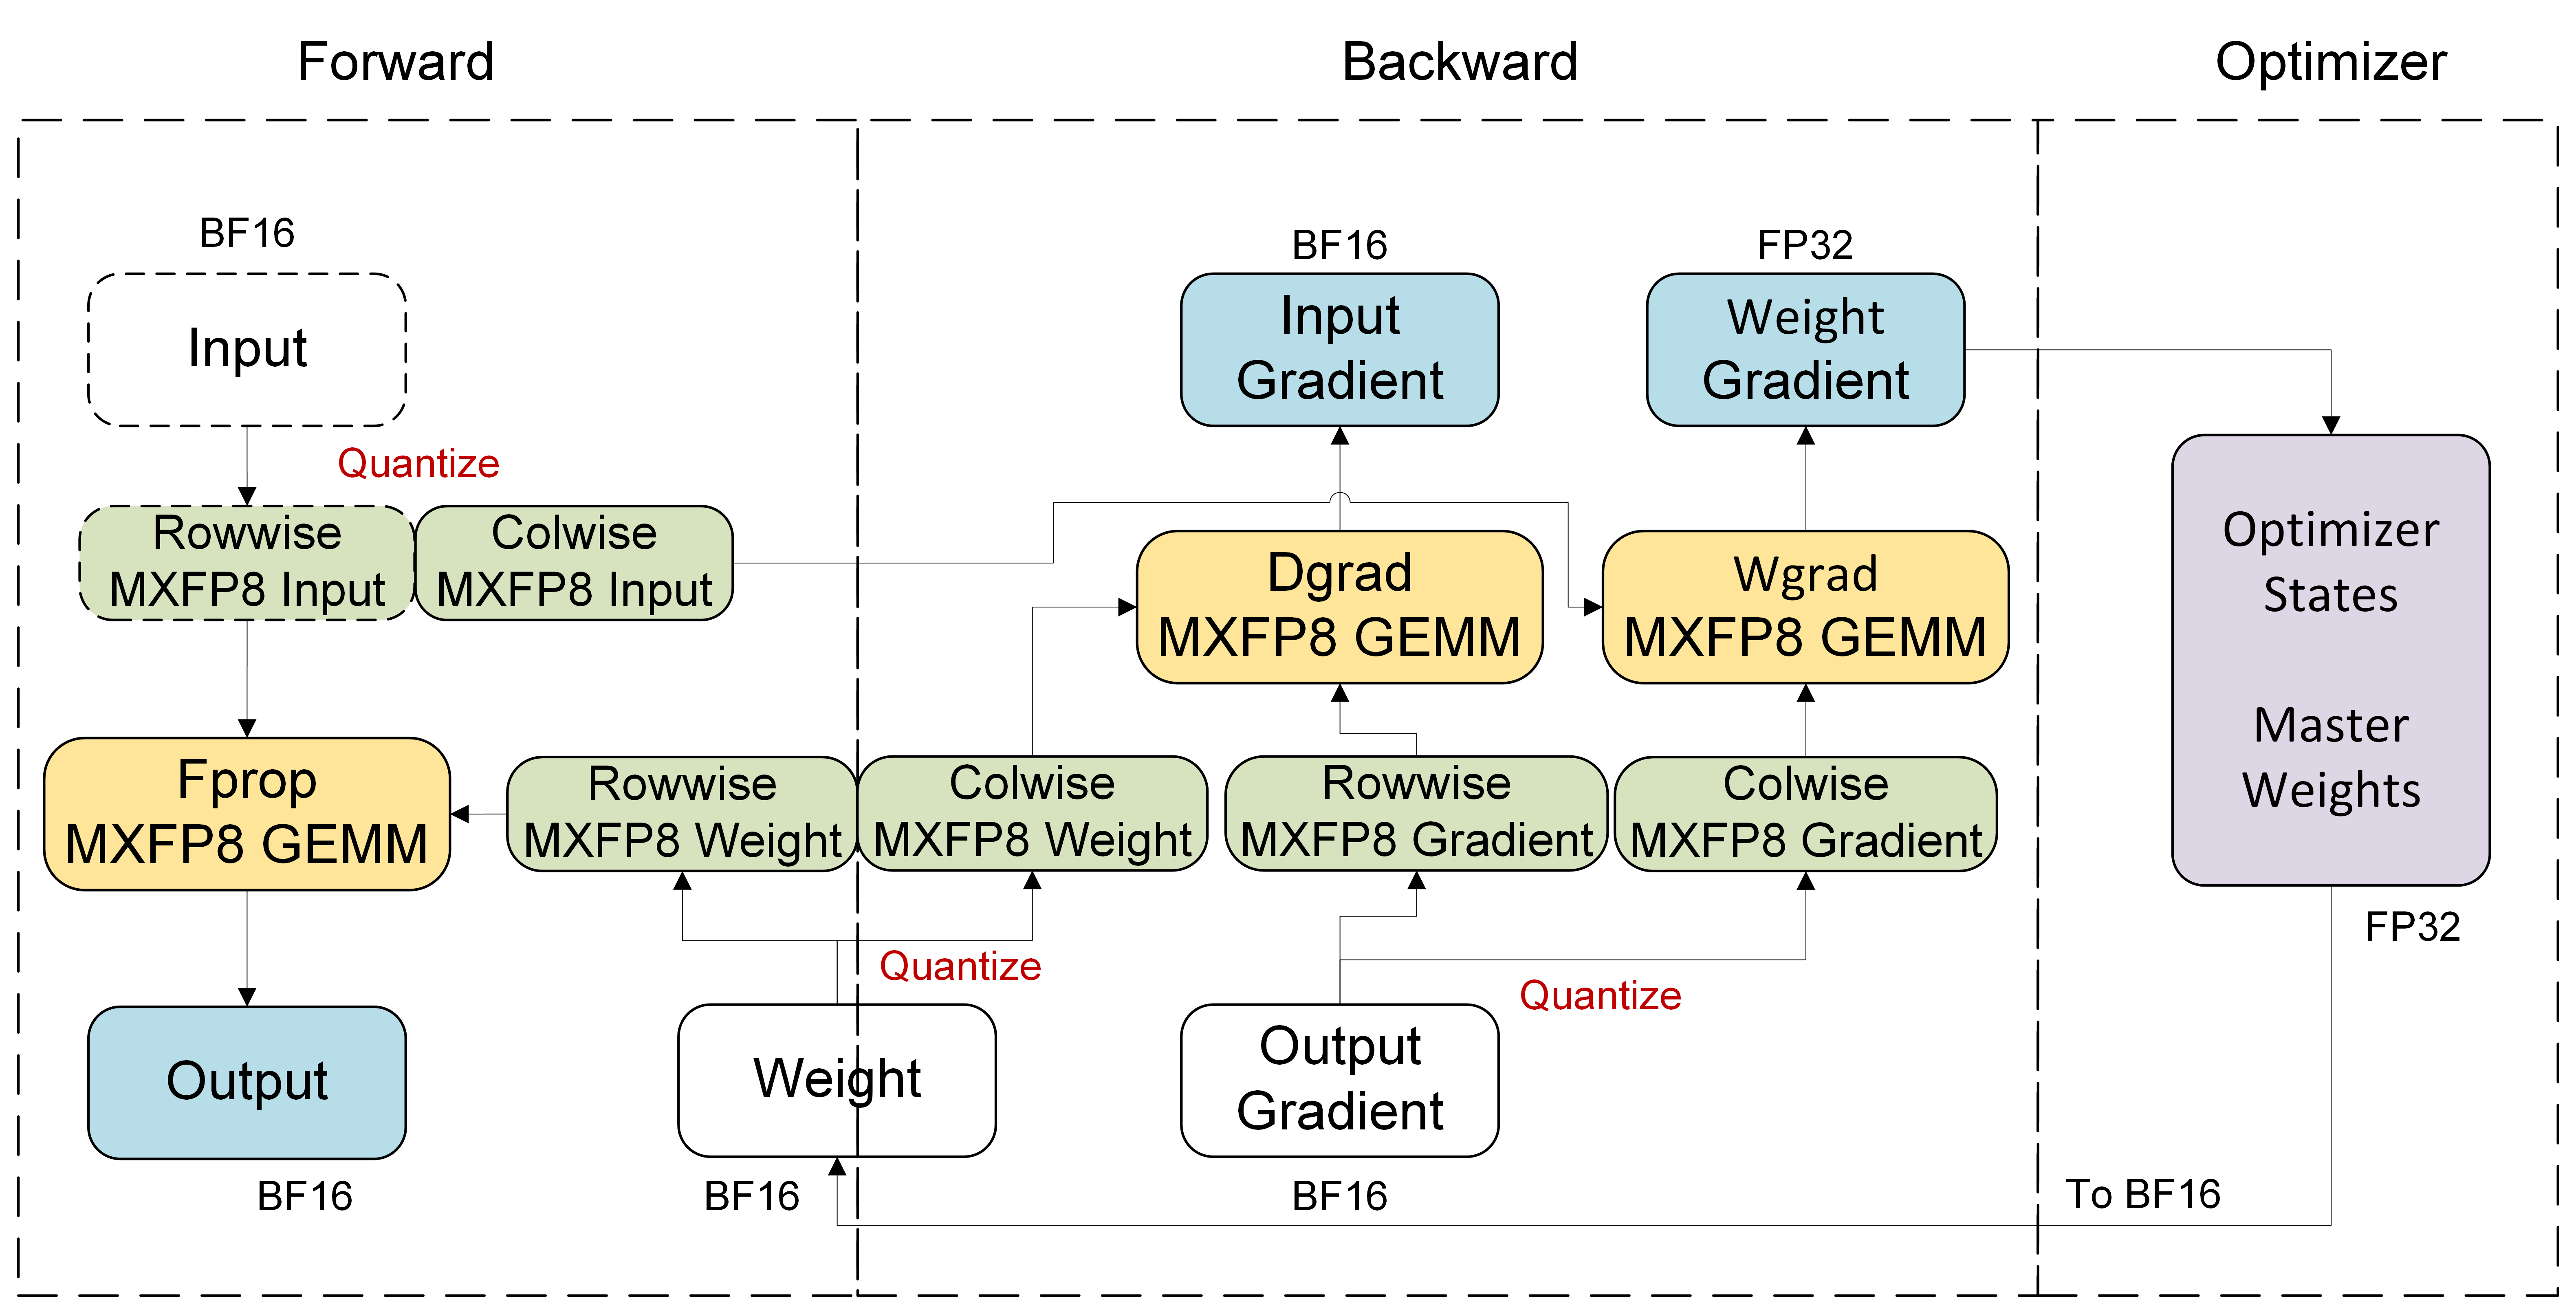
\includegraphics[width=1.0\linewidth]{figures/fp8-mxfp8.png}
        \caption{MXFP8 recipe on the Blackwell platform.}
        \label{fig:fp8-mxfp8}
    \end{subfigure}
    \caption{The computation of a linear layer with various FP8 recipes. Note the differences in quantization granularity and tensor layout requirements across platforms.}
    \label{fig:fp8-recipes}
\end{figure*}

\subsubsection{Blockwise FP8 on Hopper}
The blockwise FP8 recipe adopts the E4M3 format for all tensors, quantizing activations and gradients in $1 \times 128$ tiles and weights in $128 \times 128$ blocks. Blockwise scaling uses fine-grained scaling granularity for better precision and has been \textbf{proven successful in production} at very large-scale MoE models, including DeepSeek-V3 \cite{deepseekai2025deepseekv3technicalreport}, Minimax-M2 \cite{minimax_m2}, Ant Ling-2.0 \cite{li2025every}, etc. As a result, blockwise FP8 is the recommended FP8 recipe on the Hopper platform.

Transformer Engine provides highly optimized quantization kernels and GEMM kernels (via cuBLAS) for the blockwise recipe, as well as layer-level APIs and an autocast context to enable FP8 training with just a few lines of code.

\Figref{fig:fp8-blockwise-hopper} illustrates the computation of a linear layer with the blockwise FP8 recipe on the Hopper platform, which is very similar to the per-tensor current scaling on Hopper, except for tile-based quantization.

\subsubsection{MXFP8 on Blackwell}
On the Blackwell platform, thanks to native fifth-generation Tensor Core support for the MXFP8 format \cite{rouhani2023microscalingdataformatsdeep}, we adopt MXFP8, a more fine-grained quantization scheme for training. Both activations and weights are quantized at $1 \times 32$ granularity, and E8M0 is used for the scaling factor. Theoretically, MXFP8 should be more precise due to the finer-grained scaling granularity, and has better performance due to the native support of MXFP8 in the Tensor Core. Therefore, MXFP8 is the default FP8 recipe on the Blackwell platform.

\Figref{fig:fp8-mxfp8} illustrates the computation of a linear layer with the MXFP8 recipe on the Blackwell platform. Although FP8 GEMMs with all layouts are supported on Blackwell, we need to store additional column-wise quantized FP8 data for activations and weights due to quantization in the other direction.

Ongoing optimizations for the MXFP8 recipe in MoE training include:
\begin{enumerate}
    \item Grouped quantization to reduce the quantization overhead.
    \item Fuse activation and quantization (for the following GEMM) with the GEMM kernel.
    \item Ensure that the whole pipeline of MXFP8 quantization, scaling factor swizzling, and Grouped GEMM is CUDA-graphable.
\end{enumerate}

\subsubsection{NVFP4 on Blackwell}

In \cite{nvidia2025pretraininglargelanguagemodels}, we presented NVFP4 as a 4-bit microscaling format for LLM training that improves numerical fidelity while preserving the efficiency benefits of FP4. 

NVFP4 uses FP4 elements in E2M1 format, so values are quantized with scaling because raw FP4 has a very limited representable range. A central design choice is two-level microscaling. NVFP4 applies a per-tensor FP32 scale and a per-block 8-bit scale in E4M3. The tensor-level FP32 scale first remaps the tensor distribution into a range compatible with block scaling, and the block-level E4M3 scale then maps each block into FP4 range. NVFP4 uses blocks of 16 contiguous elements, and each block’s amax is scaled to the FP4 maximum.

Building on this format design, we also found that stable NVFP4 training depends on several algorithmic choices around quantization. In particular, we add three practical techniques:
\begin{itemize}
\item \textbf{Random Hadamard Transforms (RHT)}: Applied to weight gradient computation to reduce the impact of outliers.
\item \textbf{2D scaling}: Specifically, 16x16 weight block scaling (with the FP32 tensor scale retained) is used to keep weight quantization more consistent between forward and backward passes and reduce forward/backward quantization mismatch.
\item \textbf{Stochastic rounding}: Used on gradients to reduce rounding bias during FP4 conversion, as deterministic rounding introduces bias that hurts convergence.
\end{itemize}
These additions are a key part of the training recipe used in the paper and are important for convergence at larger scales.

\begin{figure}[ht]
    \centering
    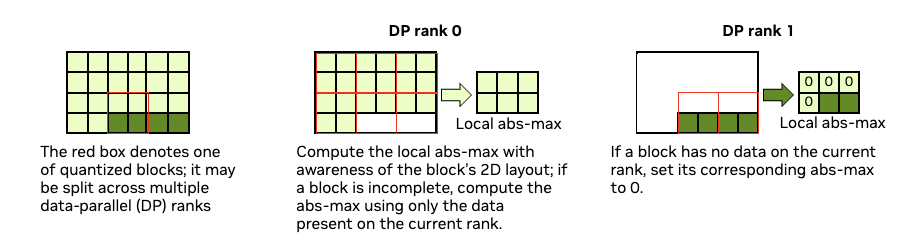
\includegraphics[width=1\linewidth]{figures/native_fp8_blockwise.png}
    \caption{FP8 primary weight quantization scheme for blockwise scaling.}
    \label{fig:native_fp8_blockwise}
\end{figure}

\subsubsection{FP8/FP4 Primary Weights: Eliminating Redundant Storage}\label{subsec:fp8-primary-weights}
Conventional reduced-precision training maintains a three-tier parameter hierarchy: FP32 master weights for optimizer updates, BF16 model weights as an intermediate representation, and FP8/FP4 weights for forward and backward GEMM computation. This introduces redundant memory overhead by maintaining both BF16 and FP8/FP4 copies of parameters.

\textbf{Native FP8/FP4} eliminates this redundancy by establishing a direct casting path from FP32 master weights to FP8/FP4 computation weights, bypassing the BF16 intermediate layer entirely, reducing memory footprint and accelerating parameter AllGather.

The core challenge in implementing native FP8/FP4 lies in managing the quantization metadata required for FP8/FP4 tensors. We provide a unified interface supporting different FP8/FP4 recipes (delayed scaling, current scaling, blockwise scaling, MXFP8 and NVFP4) that handles version-specific differences in TransformerEngine's implementations, ensuring compatibility across versions.

During each optimizer step in the distributed optimizer, the FP32 parameter shards are updated based on reduced gradients. Subsequently, these updated FP32 shards are directly quantized to FP8/FP4 format using the appropriate scaling factors. The quantization process computes the amax from the FP32 values, updates the scaling factors across data-parallel ranks to maintain consistency, and writes the quantized FP8/FP4 values to the model parameter buffers. This direct path eliminates the memory overhead of maintaining BF16 parameters, a reduction particularly impactful for large language models where parameter memory can exceed hundreds of gigabytes.

More specifically, the quantization of FP32 shards for delayed scaling and current scaling proceeds in three steps, see \figref{fig:native_fp8_current_scaling}:
\begin{itemize}
    \item Step 1: Get local abs-max from master weights. If a weight has no sharded part on the current rank, set its corresponding abs-max to 0.
    \item Step 2: Get global abs-max through AllReduce.
    \item Step 3: Use global abs-max and master weights to do partial cast.
\end{itemize}

\begin{figure}[ht]
    \centering
    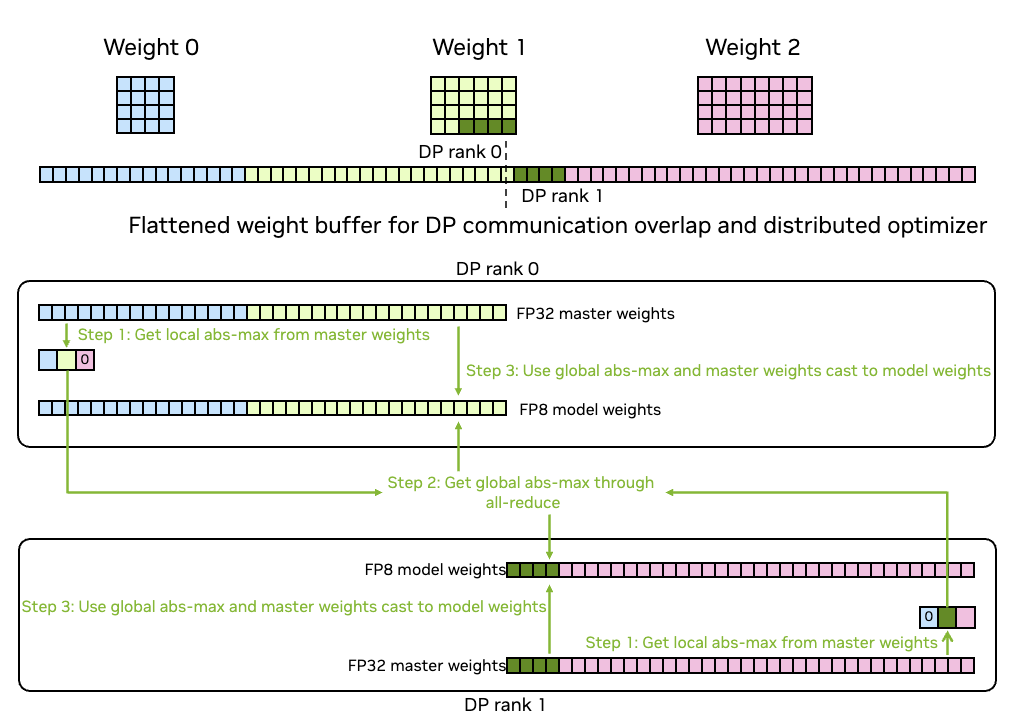
\includegraphics[width=1\linewidth]{figures/native_fp8_current_scaling.png}
    \caption{FP8 primary weight quantization scheme for delayed scaling and per-tensor current scaling.}
    \label{fig:native_fp8_current_scaling}
\end{figure}

In the Blockwise recipe, the abs-max of a weight is computed over a 2D block, so we cannot directly use a reduction kernel to obtain the local abs-max. We implemented specialized kernels that are aware of the weight's 2D layout and the correspondence between the master weight and the original weight to compute the abs-max, see \figref{fig:native_fp8_blockwise}.

Another advantage of FP8/FP4 primary weights is that the parameter AllGather communication volume is greatly reduced (see Section \ref{sec:comm_wall_quantized_training}).


\subsection{MoE-Specific Challenges and Solutions of Reduced-Precision Training}

The preceding subsections covered the fundamentals of reduced-precision training applicable to any deep learning model. MoE architectures introduce unique challenges for reduced-precision training that require specialized solutions beyond standard implementations.

\subsubsection{Fusion of Padding and Unpadding: Dynamic Shape Alignment}
FP8 and FP4 GEMMs require tensor dimensions to be aligned to specific multiples: 16 for per-tensor and blockwise recipes, and 32 for MXFP8 and NVFP4. These padding requirements arise from the block scaling granularity of each quantization recipe, as well as the requirement that Tensor Memory Accelerator (TMA) accesses maintain 16-byte alignment along the GEMM dot-product dimension. In the forward pass, the hidden dimension K is the dot-product dimension and is usually already aligned by model design. However, in the weight-gradient GEMM, the dot-product dimension corresponds to the token dimension M, which varies dynamically and often does not satisfy the alignment requirement. As a result, zero-padding along the token dimension is necessary. To further enable grouped quantization kernels with lower CPU overhead and CUDA Graph compatibility, we increase the tokens-per-expert padding to 128. Section \ref{sec:fp4-quant-fusion} explains why this larger padding is required for the NVFP4 grouped quantization kernel; the same principle also applies to MXFP8 grouped quantization. In summary, the final padding applied to the token dimension is determined jointly by the requirements of all kernels involved in the routed expert layer.

Our baseline solution is the fused padding and unpadding kernels for multiple input tensors for different experts. However, explicit padding and unpadding kernels introduce non-negligible overheads. We propose two solutions:
\begin{itemize}
    \item \textbf{Routing map padding}, which pads the routing map instead of the received tokens. This ensures the number of tokens per expert is aligned to the requirement at the cost of sending only a small number of extra tokens, avoiding expensive per-tensor padding operations.
    \item \textbf{Fusing padding into permutation} avoids one-pass of global memory read and write and should provide the best performance. It is the default choice when available.
\end{itemize}

% \subsubsection{FP8 EP Communications: Halving Dispatch Volume}\label{sec:fp8-dispatch-comm}
% With large EP strategies for fine-grained MoE models, EP communication becomes the primary bottleneck. To reduce this overhead, dispatch communication can be executed using FP8, halving the all-to-all volume.

% \textbf{Key insight}: Only the 1D per-token scaled recipe can make FP8 dispatch communication feasible (\figref{fig:fp8_dispatch}). In 1D per-token quantization, each token is associated with its own \textbf{row-wise} scaling factor tensor, which is preserved even after all-to-all communication. However, during weight gradient computation, the GEMM operation requires col-wise quantized (and optionally transposed) FP8 activations as input, which requires a dequantization and re-quantization (along another direction) step. To minimize potential accuracy loss due to double quantization, the E8M0 or power-of-two scale format is adopted.

% \begin{figure}[ht]
%     \centering
%     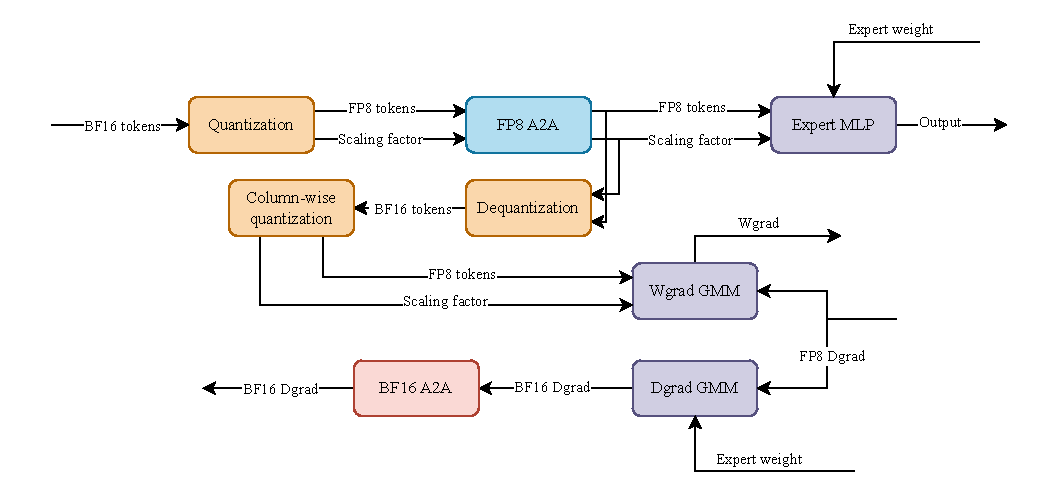
\includegraphics[width=1\linewidth]{figures/fp8_dispatch.drawio.pdf}
%     \caption{Using FP8 communication in the forward dispatch. The dequantization-quantization step is required for backward computation.}
%     \label{fig:fp8_dispatch}
% \end{figure}

% \paragraph*{Platform-Specific Implementations.}
% The blockwise recipe is used on Hopper, where FP8 GEMM only accepts inputs with a TN layout. This means the activation input must be row-major, so an additional transpose is required after column-wise quantization. In contrast, the MXFP8 recipe is employed on the Blackwell architecture, which supports arbitrary layouts and eliminates the need for this extra transpose.

% In the blockwise recipe, we need to quantize the tokens before communication. The quantized activations can directly participate in the forward computation. However, for the backward pass, we must first dequantize to reconstruct the high-precision input, then re-quantize to obtain the new result. This is because, for the same activation, the quantization dimensions used in the forward and backward phases are different. Since the Hopper Tensor Core only accepts specific layouts, a transposition step is also required beforehand.

% In the MXFP8 recipe, the process is almost identical to that of the blockwise method. Though transposition is unnecessary on the Blackwell platform, we still need the FP8 tensor quantized along different dimensions (col-wise vs. row-wise) for backward computation.

\subsubsection{Grouped Quantization and Grouped GEMM}

\paragraph{Grouped Quantization}

Due to the different padding requirements between the quantized data and scaling factors, and the complex data layouts introduced by both row-wise and column-wise quantization, a naive way to quantize the input tensors for different experts is to apply the quantization kernel to them one by one. Nevertheless, it introduces plenty of tiny kernels, which adds to the CPU overhead and is not efficient from the GPU perspective.

To tackle this problem, we implement grouped quantization kernels to fuse the quantization of multiple tensors into one single kernel, which greatly reduces the CPU overhead, improves the GPU utilization and is CUDA-Graphable.

\paragraph{Grouped GEMM}
Optimized and CUDA-Graphable grouped GEMM in Section \ref{sec:device-init}.


\subsubsection{NVFP4 Quantization Fusion}\label{sec:fp4-quant-fusion}

NVFP4 quantization is particularly more complicated because of the numerical techniques we use to preserve numerical stability, so aggressive kernel fusion is necessary to keep quantization overhead under control. In practice, our NVFP4 quantization kernel is not just a simple “scale + cast” kernel: it needs to carefully absorb the training-recipe logic, including Random Hadamard Transform, 2D scaling and stochastic rounding. 

Among these, RHT fusion is the most latency-sensitive. If implemented as a separate kernel, the Hadamard transform would introduce an additional full-precision (BF16) read/write of the tensor in global memory, significantly increasing bandwidth cost. By fusing RHT with NVFP4 quantization, we perform the Hadamard transform and FP4 quantization in a single kernel, avoiding that extra BF16 traffic.

A second implementation challenge is that Blackwell NVFP4 Tensor Core GEMMs are TN-oriented, while Wgrad uses transposed activations and gradients. Therefore, when RHT is fused into NVFP4 quantization for the Wgrad path, the kernel must also absorb the transpose, rather than relying on a separate BF16 transpose kernel (which would again incur a full BF16 tensor read and write through global memory).

As a result, the fused quantization pipeline must support multiple outputs from the same high-precision input: (1) standard FP4 quantization for forward-pass GEMMs, and (2) transpose + RHT + FP4 quantization for the backward/Wgrad path. In training, we launch this fused kernel during the forward pass to generate two FP4 copies: one consumed immediately by the forward GEMM, and one saved for backward. The original high-precision input is then discarded, so we avoid storing BF16 activations while still preparing the backward path efficiently.

A further complication comes from the per-tensor FP32 scale in NVFP4. Current NVFP4 pretraining recipe, the tensor-wide abs-max is measured after the Hadamard transform, which means we need a dedicated Hadamard+amax kernel that computes only the amax (without materializing a transformed BF16 output buffer). As a result, the Hadamard transform is effectively computed twice—first in the Hadamard-amax kernel and then again in the fused quantization kernel. Although this duplicates transform compute, it is still faster end-to-end than writing out a full transformed BF16 tensor to global memory, because it avoids the extra high-bandwidth BF16 read/write traffic.

In contrast, 2D quantization is less visible in end-to-end throughput because it applies only to weights: we can quantize weights once (for example, on the first microbatch) and cache the quantized weights and scales for reuse across later microbatches, so its cost is largely amortized. 

Stochastic rounding, however, adds a kernel-level requirement on the critical path: the quantization kernel must also support an optional stochastic rounding path with random number generated in kernel (enabled for gradient tensors such as dY, disabled otherwise) so that FP4 quantization remain fused in a single pass. To keep this efficient, we use NVIDIA cuRANDDx\cite{curanddx} for device-side random number generation inside the fused CUDA quantization kernel.

\paragraph{Grouped NVFP4 Quantization for MoE}

Supporting NVFP4 quantization for MoE layers is especially challenging due to the algorithmic complexity of the NVFP4 recipe itself. Under a full-iteration CUDA Graph requirement, the MoE quantization path must also be CUDA Graph safe: the host cannot depend on dynamic expert-token counts on the CPU, and can only rely on a device-side tokens-per-expert tensor. This means that input activation can no longer be splitted and quantized individually. We must implement grouped quantization kernels for the full NVFP4 pipeline. The memory allocation of NVFP4 output must be allocated as a whole flat buffer without knowing the shapes in between. 

A key observation is that much of the dense NVFP4 activation quantization kernel can be reused for grouped quantization, because tokens for different experts are continuously packed in memory after routing/permutation. The main differences are implementation constraints needed to preserve performance and graph safety. 

\begin{enumerate}

\item A quantization thread block should not span tokens from multiple experts, since that introduces significant control-flow and indexing overhead; therefore, we zero-pad each expert’s token count to an integer multiple of the thread block shape in the token dimension (typically 128). 

\item The NVFP4 transpose must be performed per expert (transpose each expert’s packed activation independently, then concatenate), which is not equivalent to transposing the entire grouped buffer as one tensor. 

\item NVFP4 GEMM requires scale-factor swizzling: scaling factors must be padded to a 128×4-aligned shape and swizzled into the 32×16 layout before GEMM as described in the cuBLAS document\cite{cublas_sf_layout}. This scaling factor shape constraint is applied to per-expert GEMM, which means that determining the required padding size would implicitly require CPU visibility into tokens-per-expert, which is not CUDA Graph safe. To avoid that, we enforce 128-token alignment per expert by construction.
\end{enumerate}

Both point 1) and point 3) imposed 128 multiple tokens-per-expert, which requires a specific zero padding kernel to satisfy. To eliminate such zero padding overhead, we fuse the per-expert zero-padding capability into the token-permute kernel, so the routed expert activations are produced in an already aligned and zero padded layout, and downstream grouped NVFP4 quantization/GEMM kernels can assume the required alignment without additional preprocessing.

For the per-tensor FP32 second-level scale in the NVFP4 recipe, the per-tensor second-level scale in MoE means per-expert second-level scale instead of making every expert share the amax to preserve numerical stability during training. These amax values cannot be known ahead of time: they must be computed online from the routed tokens and generated as distinct per-expert amax values on every iteration. To address this efficiently, we leverage the 128-aligned tokens-per-expert guarantee and adapt the dense-input implementation into a CUDA-Graph-safe grouped Hadamard-amax kernel. 

%==============================================================================
% SECTION 6: LONG-CONTEXT MOE TRAINING
%==============================================================================

